\chapter{A multigrid preconditioned conjugate gradients algorithm for large voxelized Poisson problems}\label{chap:poisson}
\begin{figure*}[ht]
\center{
 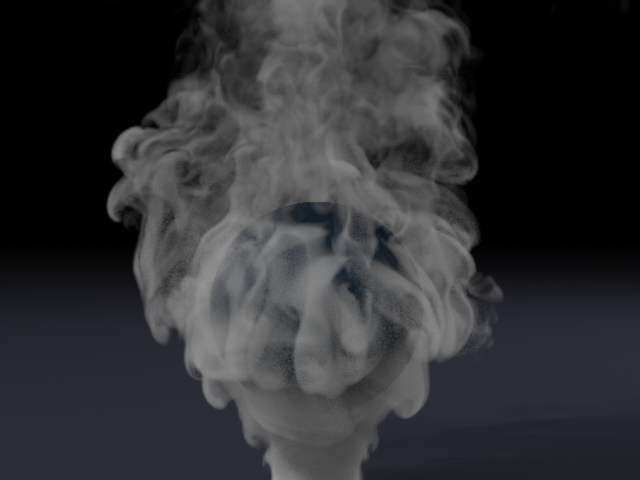
\includegraphics[width=.32\textwidth]{poisson/figures/smoke_768_closeup_00144.png}
 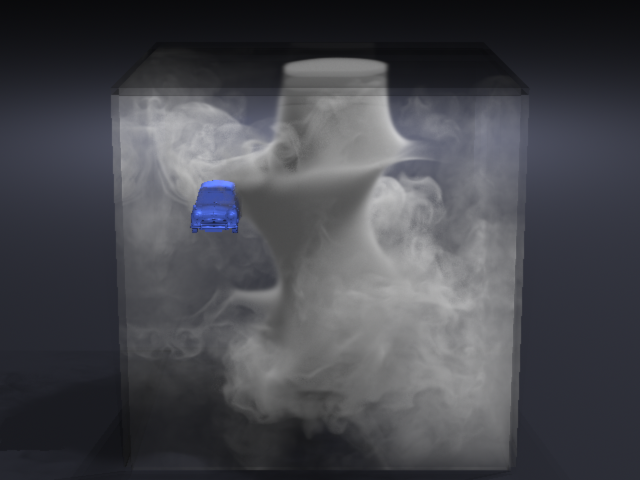
\includegraphics[width=.32\textwidth]{poisson/figures/smoke_car_768_00223.png}
 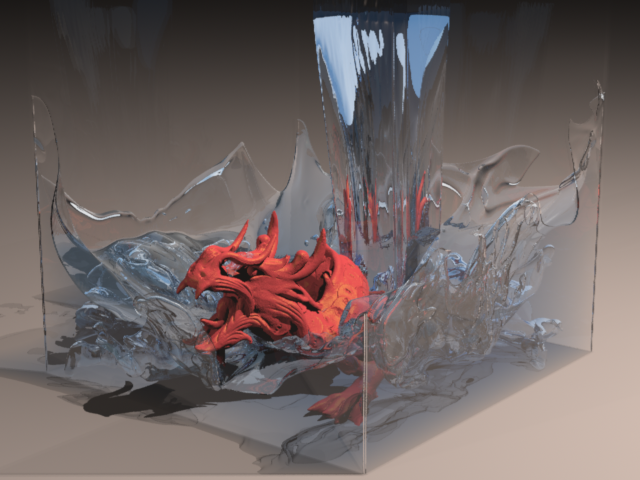
\includegraphics[width=.32\textwidth]{poisson/figures/dragon_deep_pool_00084.png}
}
 \caption{Left: Simulation of smoke flow past a sphere, at $768^2\!\times\!1152$ resolution (close-up view). Middle: A column of smoke is stirred up by a revolving object -- $768^3$ resolution. Right: Free
   surface simulation of water poured on a dragon figurine at $512^3$ resolution.}
\end{figure*}


%\section{Introduction}
%Incompressible flows have proven very effective at generating many compelling effects in computer graphics including free surface, multiphase and viscoelastic fluids, smoke and fire. 
%One
%of the most popular techniques for enforcing the incompressibility constraint is MAC grid based projection as pioneered by \cite{HW65}. They showed that for simulations on a regular
%Cartesian lattice, staggering velocity components on cell faces and pressures at cell centers gives rise to a natural means for projecting such a staggered velocity field to a discretely
%divergence free counterpart. This projection is ultimately accomplished by solving a Poisson equation for the cell centered pressures. Categorization of the Cartesian domain into air,
%fluid or solid cells gives rise to what \cite{BBB07} describe as the ``voxelized Poisson equation'' with unknown pressures and equations at each fluid cell, Dirichlet boundary conditions
%in each air cell and Neumann boundary conditions at faces separating fluid and solid cells. This technique for enforcing incompressibility via voxelized Poisson was originally
%popularized in computer graphics by \cite{Foster:1996:RAO} who used Successive Over Relaxation (SOR) to solve the system. \cite{FF01} later showed that incomplete Cholesky preconditioned conjugate
%gradient (ICPCG) was more efficient. This has since become a very widely adopted approach for voxelized Poisson and has been used for smoke \cite{SRF05,MTPS04,FSJ01} and fire \cite{HG09} as well as continuum models for solids such as sand \cite{ZB05} and hair \cite{MSWST09}. The voxelized pressure Poisson equation is also popular in free surface flows due to its efficiency and relative simplicity
%\cite{CMT04,FF01,GBO04,HK05,HLYK08,KC07,MTPS04,NNSM08,WMT05,ZB05}. There are alternatives to voxelized Poisson, e.g., \cite{BBB07} used a variational approach that retains the same sparsity of discretization while improving behavior on coarse grids for both smoke and free surface. Also, many non-MAC grid based approaches have been used to enforce incompressibility, typically for smoke rather than free surface simulations. For example, \cite{MCPTD09,KFCO06,FOK05,ETKSD07} use conforming tetrahedralizations to accurately enforce boundary conditions, \cite{LGF04} uses adaptive octree-based discretization, and \cite{CNF07} makes use of tetrahedralized volumes for free surface flow.
%
%Incomplete Cholesky preconditioned CG remains the state of the art for voxelized Poisson; however, at high resolutions, it becomes impractical due to the cost of recomputing the preconditioner as the domain changes and the increased number of PCG iterations needed to reduce the residual on large grids.  
%Although ICPCG certainly offers an acceleration over unpreconditioned CG, it is still impractical at high resolutions since the required number of iterations increases drastically with the size of the problem, and the cost of updating and explicitly storing the preconditioner (a principally non-parallel construction process) 
%is very high for large domains.  Furthermore, since ICPCG involves sparse back-substitution, it cannot be parallelized without further modification \cite{Hughes:2007:physicalsimulation}.
%Whereas multigrid methods have the potential for constant asymptotic convergence rates, our purely geometric multigrid preconditioned conjugate gradient algorithm is the \emph{first} in the graphics literature to demonstrate these convergence rates on the highly irregular voxelized domains common to free surface simulation.

%\section*{Our main contributions}
%\vspace*{-4pt}

% \noindent$\bullet$  We solve for the true solution of the voxelized Poisson equation at full resolution.  A number of recent works have focused on alternative simplified approximations to enforce incompressibility, citing the bottleneck of solving the Poisson equation at high resolutions \cite{HG09}.   Our method allows us to efficiently solve for incompressibility via pressure projection on large grids, effectively eliminating the bottleneck, and we demonstrate the effectiveness of our technique when applied to high resolution fluid simulations.  

We handle an \emph{arbitrary mix of Dirichlet and Neumann boundary conditions} on \emph{irregular voxelized domains} common to free surface flow simulations. Previous works proposing geometric multigrid methods for rectangular domains \cite{TO94,AF96,BWR05,BWK06,KH08}, as well as irregular Neumann boundaries (via a projection method) \cite{MCPN08}, cannot handle this general case.  

We use a \emph{purely geometric, matrix-free formulation} and \emph{maintain constant convergence rates}, regardless of boundary geometry.  \cite{BWR05} presents a lightweight, matrix-free geometric multigrid method for uniform rectangular domains; however, extension to voxelized domains has proved challenging.  In fact, \cite{HMB05} chose a cut-cell embedded boundary discretization, citing non-convergence on the voxelized Poisson discretization due to instabilities at irregular boundaries.  Even higher order embeddings do not ensure constant convergence as noted by \cite{CLB09}, where they solve the Poisson equation on a surface mesh embedded in a background lattice: they noticed convergence deterioration when the coarse grid could not resolve the mesh.  Furthermore, a number of works have opted to use the more general algebraic multigrid, despite its significantly greater set-up costs and difficult to parallelize nature\cite{trottenberg:2001:multigrid}, due to the challenges of finding a convergent geometric solution \cite{CNF07, CGR04, PM04}.

In comparison to widely-used ICPCG solvers, our method \emph{requires less storage, is more convergent, and more parallelizable}.  Unlike ICPCG, no preconditioning matrices are explicitly stored.  This allows us to accommodate as many as $768^2\!\times\!1152$ voxels with less than $16$GB of memory. Whereas ICPCG requires sparse backsubstition and cannot be parallelized without significant modifications, this is not the case for our solver.  Finally, we demonstrate that our solver is significantly faster than ICPCG on moderately sized problems, and our convergence rates are independent of grid size, so this performance comparison improves with resolution.  As a result, we can solve (with residual reduction by a factor of $10^4$) at $128^3$ resolution in less than $0.75$ seconds and $768^3$ resolution in about a minute.

% \vspace*{-.05in}
\section{Related Work}
% \vspace*{-.05in}

Incomplete Cholesky preconditioned CG remains the state of the art for voxelized Poisson; however, at high resolutions, it becomes impractical due to the cost of recomputing the preconditioner as the domain changes and the increased number of PCG iterations needed to reduce the residual on large grids.  
Although ICPCG certainly offers an acceleration over unpreconditioned CG, it is still impractical at high resolutions since the required number of iterations increases drastically with the size of the problem, and the cost of updating and explicitly storing the preconditioner (a principally non-parallel construction process) 
is very high for large domains.  Furthermore, since ICPCG involves sparse back-substitution, it cannot be parallelized without further modification \cite{Hughes:2007:physicalsimulation}.
Whereas multigrid methods have the potential for constant asymptotic convergence rates, our purely geometric multigrid preconditioned conjugate gradient algorithm is the \emph{first} in the graphics literature to demonstrate these convergence rates on the highly irregular voxelized domains common to free surface simulation.

Multigrid methods have proven effective for a number of applications in graphics including image processing \cite{KH08,BWK06,RC03}, smoke simulation \cite{MCPN08}, mesh deformation \cite{SYBF06}, thin shells \cite{green:2002:subdivision}, cloth simulation \cite{Oh:2008:APF}, fluid simulation \cite{CNF07,CTG10}, geometry processing \cite{ni:2004:multigrid}, deformable solids simulation \cite{OGR07}, rendering \cite{Stam95multiplescattering,HMB05}, and have been efficiently ported to the GPU \cite{BFGS03,goodnight:2003:multigrid,GSMMWBT08}. While the majority of works in this area either focused on rectangular domains or algebraic multigrid formulations on irregular geometries, there are some notable geometric multigrid solutions for irregular domains. \cite{HMB05} and \cite{CLB09} embed their irregular geometry into regular lattices, producing irregular stencils. \cite{RC03,Oh:2008:APF} use a coarse-to-fine geometric hierarchy which ensures mesh alignment across levels, but these methods require the geometry to be fully resolved at the coarsest level and thus are impractical for resolving fine fluid features.   \cite{SAB99} show that using multigrid as a preconditioner to CG rather rather than a stand-alone solver can alleviate instability issues on some problems.  Multigrid preconditioned CG for the Poisson equation on rectangular grids can be found in \cite{T93} and the algorithm is parallelized in \cite{TO94} and later \cite{AF96}.  \cite{KH08} introduced a higher-order parallel multigrid solver for large rectangular images. 
% 
% For high resolution fluid simulations, incomplete Cholesky preconditioned CG can be impractical due the cost of recomputing the preconditioner as the domain changes and the large number of
% PCG iterations needed to sufficiently reduce the residual on large grids. Multigrid methods can alleviate these issues and are in fact algorithmically optimal for a wide
% range of discrete elliptic PDE \cite{trottenberg:2001:multigrid}, and \cite{BWR05} developed a matrix-free geometric multigrid algorithm for the Poisson equation on uniform grids which required less memory than CG.  \cite{T93} showed that multigrid as a preconditioner to CG on regular domains retains this optimal convergence and demonstrated it on distributed memory machines \cite{TO94}.   These methods have proven effective for a number of applications in graphics including image processing \cite{KH08,BWK06,RC03},
% smoke simulation \cite{MCPN08}, mesh deformation \cite{SYBF06}, thin shells \cite{green:2002:subdivision}we, cloth simulation \cite{Oh:2008:APF}, fluid simulation \cite{CNF07}, geometry processing \cite{ni:2004:multigrid}, deformable solids simulation \cite{OGR07}, rendering \cite{Stam95multiplescattering,HMB05}, and have been efficiently ported to the GPU \cite{BFGS03,goodnight:2003:multigrid,GSMMWBT08}. 
% 
% Unfortunately, these methods can be difficult to perfect in the presence of irregular/rapidly changing computational domains characteristic of fluid computations.  As noted by \cite{HMB05,PM04,CNF07}, difficulties arise when devising geometric coarsening strategies on irregular domains, and improper boundary treatment can easily lead to suboptimal convergence or even divergent results.  Certain remedies have been proposed, for example \cite{MCPN08} use multigrid methods together with a boundary projection to facilitate GPU accelerated discretization of the voxelized Poisson equation for smoke, although this approach is not designed for free surface. When solving the Poisson equation over the surface of a mesh, \cite{CLB09} restrict a mesh-independent space of functions with a geometric coarsening strategy to their surface mesh; however, they found that convergence was slowed when the coarse resolution space did not closely match the mesh geometry.  In some applications, it is possible to use a coarse-to-fine geometric hierarchy which ensures mesh alignment across levels \cite{RC03,Oh:2008:APF}, but these methods require the geometry to be fully resolved at the coarsest level and thus are impractical resolving fine fluid features.  Since algebraic multigrid methods construct their hierarchy from the operator matrix, they can be seen as black-box solvers and have been used to circumvent the geometric coarsening complications \cite{CNF07, CGR04, PM04}. However, this robustness comes at significant set-up and memory cost as coarse grid matrices must be explicitly computed and stored \cite{trottenberg:2001:multigrid}.  Our geometric multigrid preconditioned CG method for the voxelized Poisson equation is lightweight without sacrificing convergence even on highly irregular domains.

% 
% \emph{Our main contributions are:}
% \begin{itemize}
% %% \vspace*{-.05in}
% \item A multigrid PCG solver for the voxelized Poisson equation capable of handling Dirichlet and Neumann conditions on
%   arbitrary irregular domains, with significantly improved efficiency over the traditional incomplete Cholesky preconditioner.
% %% \vspace*{-.05in}
% \item We detail how the preconditioner can be implemented as an optimized lightweight multigrid cycle incurring a very modest storage and computation overhead and enabling simulation of
%   very high resolution fluids on commodity workstations.
% %% \vspace*{-.05in}
% \item We demonstrate the performance of our solver on smoke and free surface simulations with resolutions up to $768^2\!\times\!1152$.
% \end{itemize}


%% We present a multigrid preconditioner and streamlined conjugate gradient method for voxelized Poisson that is accurate and efficient enough to increase performance over the traditional
%% incomplete Cholesky preconditioned method by orders of magnitude. Its simplicity naturally facilitates parallelization with a memory footprint small enough to admit extremely efficient
%% simulation on very large grids. We show that multigrid preconditioned conjugate gradient can simplify the requirements of the components of the multigrid algorithm. We adopted this
%% strategy to obtain an efficient and lightweight approach in the presence of changing and irregular geometry. We demonstrate the performance of our solver with smoke and free surface
%% fluid simulations using approximately $10^8$ voxels. Notably, we use simple semi-Lagrangian advection \cite{S99} for smoke density and level sets. This low order approach to advection is
%% often improved with Lagrangian techniques \cite{EMF02,SRF05} or vorticity confinement \cite{FSJ01} at low resolution, however we did not use them given the resolutions admitted by our
%% approach (although they should provide even more detailed dynamics).

%% There are many other alternatives to MAC based voxelized Poisson for enforcing incompressibility. However, most are not designed for free surface simulations. For example, \cite{MCPN08}
%% use multigrid methods to facilitate GPU accelerated discretization of the voxelized Poisson equation for smoke, \cite{BBB07} use a variational alternative to the voxelized Poisson
%% equation that retains the same sparsity of discretization while improving behavior on coarse grids for both smoke and free surface.


% \vspace*{-.05in}
\section{Method overview}
% \vspace*{-.05in}

We wish to solve the Poisson boundary value problem:
\begin{eqnarray}
\Delta p=f&\mbox{in}&\Omega\subset\mathbf{R}^3\\
p(\vec{x})=\alpha(\vec{x})\ \ \mbox{on}\ \ \Gamma_D\label{eqn_problem},&&p_n(\vec{x})=\beta(\vec{x})\ \ \mbox{on}\ \ \Gamma_N\nonumber
\end{eqnarray}
where the boundary of the domain $\partial\Omega=\Gamma_D\cap\Gamma_N$ is partitioned into the disjoint subsets $\Gamma_D$ and $\Gamma_N$ where Dirichlet and Neumann conditions are
imposed, respectively. For fluids simulations, $\Omega$ corresponds to the body of water, while
Dirichlet boundary conditions are imposed on the air-water interface and Neumann conditions at the surfaces of contact between the fluid and immersed objects (or the walls of
a container). Without loss of generality we will assume that the Neumann condition is zero ($\beta(\vec{x})$$=$$0$) since non-zero conditions can be expressed by modifying
the right hand side.

%%  An example is illustrated in Figure \ref{fig_domain_illustration} (left), where a volume of water is shown with a free surface, in addition to one fully immersed and
%% one partially immersed object. The values of the boundary conditions for the purposes of the pressure projection would be zero, for both Dirichlet and Neumann boundaries,
%% i.e. $\alpha(\vec{x})$$=$$0$ and $\beta(\vec{x})$$=$$0$ respectively. Our method fully supports arbitrary non-zero boundary conditions as well; however, we will momentarily assume that
%% the Neumann condition is zero ($\beta(\vec{x})$$=$$0$) for our initial exposition, and will later explain how we can trivially accommodate any other non-zero Neumann condition.

\begin{figure}[t]
\center{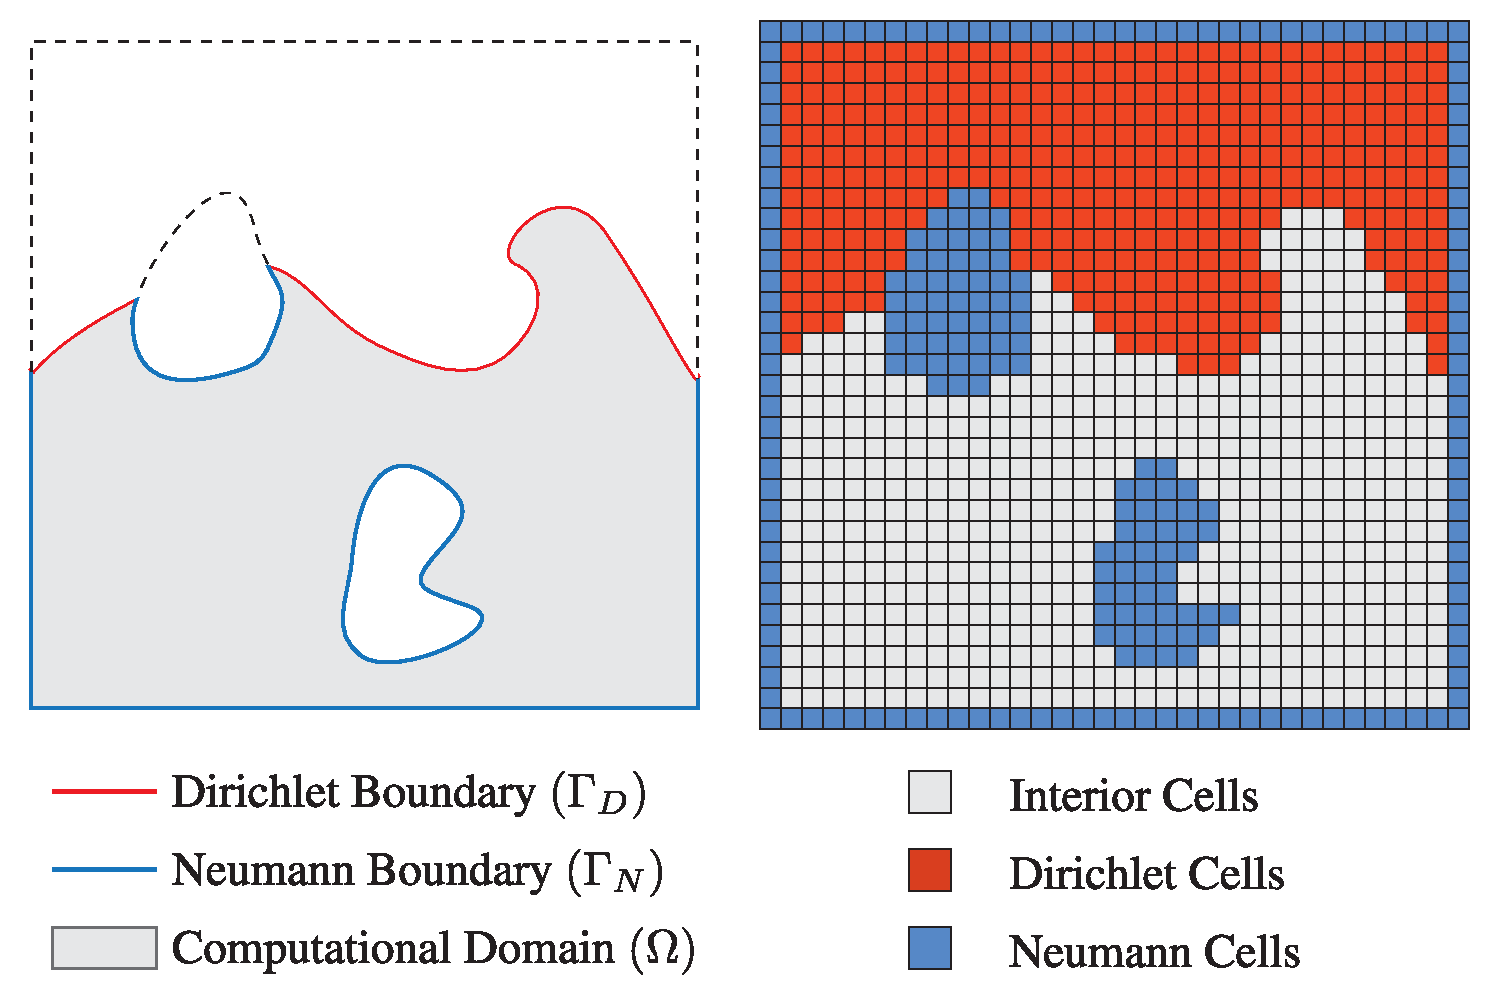
\includegraphics[width=\columnwidth]{poisson/figures/domain_illustration.pdf}}
\caption{Left: Example of the geometry for a Poisson problem. Right: Our voxelized representation of this computational domain.}
%% \vspace*{-.15in}
\label{fig_domain_illustration}
\end{figure}

%\vspace*{-.05in}
\subsection{Discretization}
\label{sec_discretization}
%\vspace*{-.05in}
We discretize the Poisson equation on a uniform Cartesian lattice, and store the unknown pressure variables $p_{ijk}$ at the cell centers of this lattice. In our approach, both the computational
domain and boundary conditions are defined at the resolution of this background lattice. In particular, the computational domain is represented as a collection of grid cells
(or voxels), which we refer to as \emph{interior cells} (colored gray in the example of Figure \ref{fig_domain_illustration}, right).
%% This voxelized approximation of $\Omega$ is a
%% commonly accepted practice in graphics, even more so at the very high resolutions we can accommodate; other options are discussed in Section \ref{sec_discussion}.
We express boundary conditions in a volumetric, voxel-based fashion. Specifically, we define Dirichlet conditions on a voxelized volumetric region, instead of imposing them strictly
along $\partial\Omega$. We label the cells in this region as \emph{Dirichlet cells} (colored red in Figure \ref{fig_domain_illustration}, right).
%% It is typically straightforward to define a volumetric extent for this Dirichlet region, e.g. for a free-surface water simulation the entire air region would be labeled as Dirichlet. Since only the values of Dirichlet
%% cells immediately adjacent to the interior region will influence our computed solution, those are the only values that need to be provided, i.e. no extrapolation of the Dirichlet
%% condition is necessary.
We similarly define regions of \emph{Neumann cells} (shown in blue in Figure \ref{fig_domain_illustration}) by rasterizing solid objects and container walls onto
the grid. Since pressures are cell-centered, Neumann conditions are naturally imposed at the cell faces between interior and Neumann cells. For simplicity of implementation, as
detailed in Section \ref{sec_implementation}, we always assume a ``ghost'' layer of Neumann cells surrounding our computational domain, as illustrated in Figure
\ref{fig_domain_illustration}. This assumption does not hinder generality since any configuration (e.g., a box with all Dirichlet boundaries) can be trivially padded with an extra layer of
Neumann cells without affecting the solution on $\Omega$.
For every interior cell we construct a discrete Poisson equation as:
\begin{equation}
\sum_{(i'\!,j'\!,k')\in\mathcal{N}^{\ast}_{ijk}}\!\!\!\!\!\!\!\!\frac{p_{i'\!j'\!k'}-p_{ijk}}{h^2}=f_{ijk}
\label{eqn_discrete_poisson}
\end{equation}
 \vspace*{-.2in}
\begin{align*}
\mathcal{N}_{ijk}&=\left\{(i\pm 1,j,k),(i,j\pm 1,k),(i,j,k\pm 1)\right\} \\
\mathcal{N}^{\ast}_{ijk}&=\left\{(i'\!,j'\!,k')\in\mathcal{N}_{ijk}:\mbox{cell}(i'\!,j'\!,k')\ \mbox{is \emph{not} Neumann}\right\}
\end{align*}
In this definition, $\mathcal{N}_{ijk}$ are the 6 neighboring cells across the faces of the interior cell $(i,j,k)$, $\mathcal{N}_{ijk}^{\ast}$ is the subset of
$\mathcal{N}_{ijk}$ that excludes any Neumann neighbor cells, and $h$ is the grid step size. Equation (\ref{eqn_discrete_poisson}) is derived from the
standard 7-point Poisson finite difference stencil using the zero-Neumann boundary condition $(p_{i'\!j'\!k'}\!-\!p_{ijk})/h\!=\!0$ to eliminate pressure values at Neumann cells from the
discrete equations.  
%In the case of inhomogeneous Neumann boundary conditions $(p_{i'\!j'\!k'}\!-\!p_{ijk})/h\!=\!\beta(\vec{x})$, this value is transferred to the right hand side. 
Away from the boundary of $\Omega$ this yields the standard 7-point stencil. Note that this formulation is identical to \cite{Foster:1996:RAO,FF01}.
%% Equation (\ref{eqn_discrete_poisson}) can be written collectively for the
%% entire domain as $\mathcal{L}\vec{p}=\vec{f}$ or $\mathcal{L}^I\vec{p}^I+\mathcal{L}^D\vec{p}^D=\vec{f}$, where $\vec{p}^I$, $\vec{p}^D$ are the pressure variables on interior and
%% Dirichlet cells respectively. Since $\vec{p}^D$ is given via the Dirichlet conditions, our problem reduces to the symmetric negative definite system
%% $\mathcal{L}^I\vec{p}^I=\vec{f}-\mathcal{L}^D\vec{p}^D$.

\begin{figure}[t]
\center{\hspace*{-.025\columnwidth}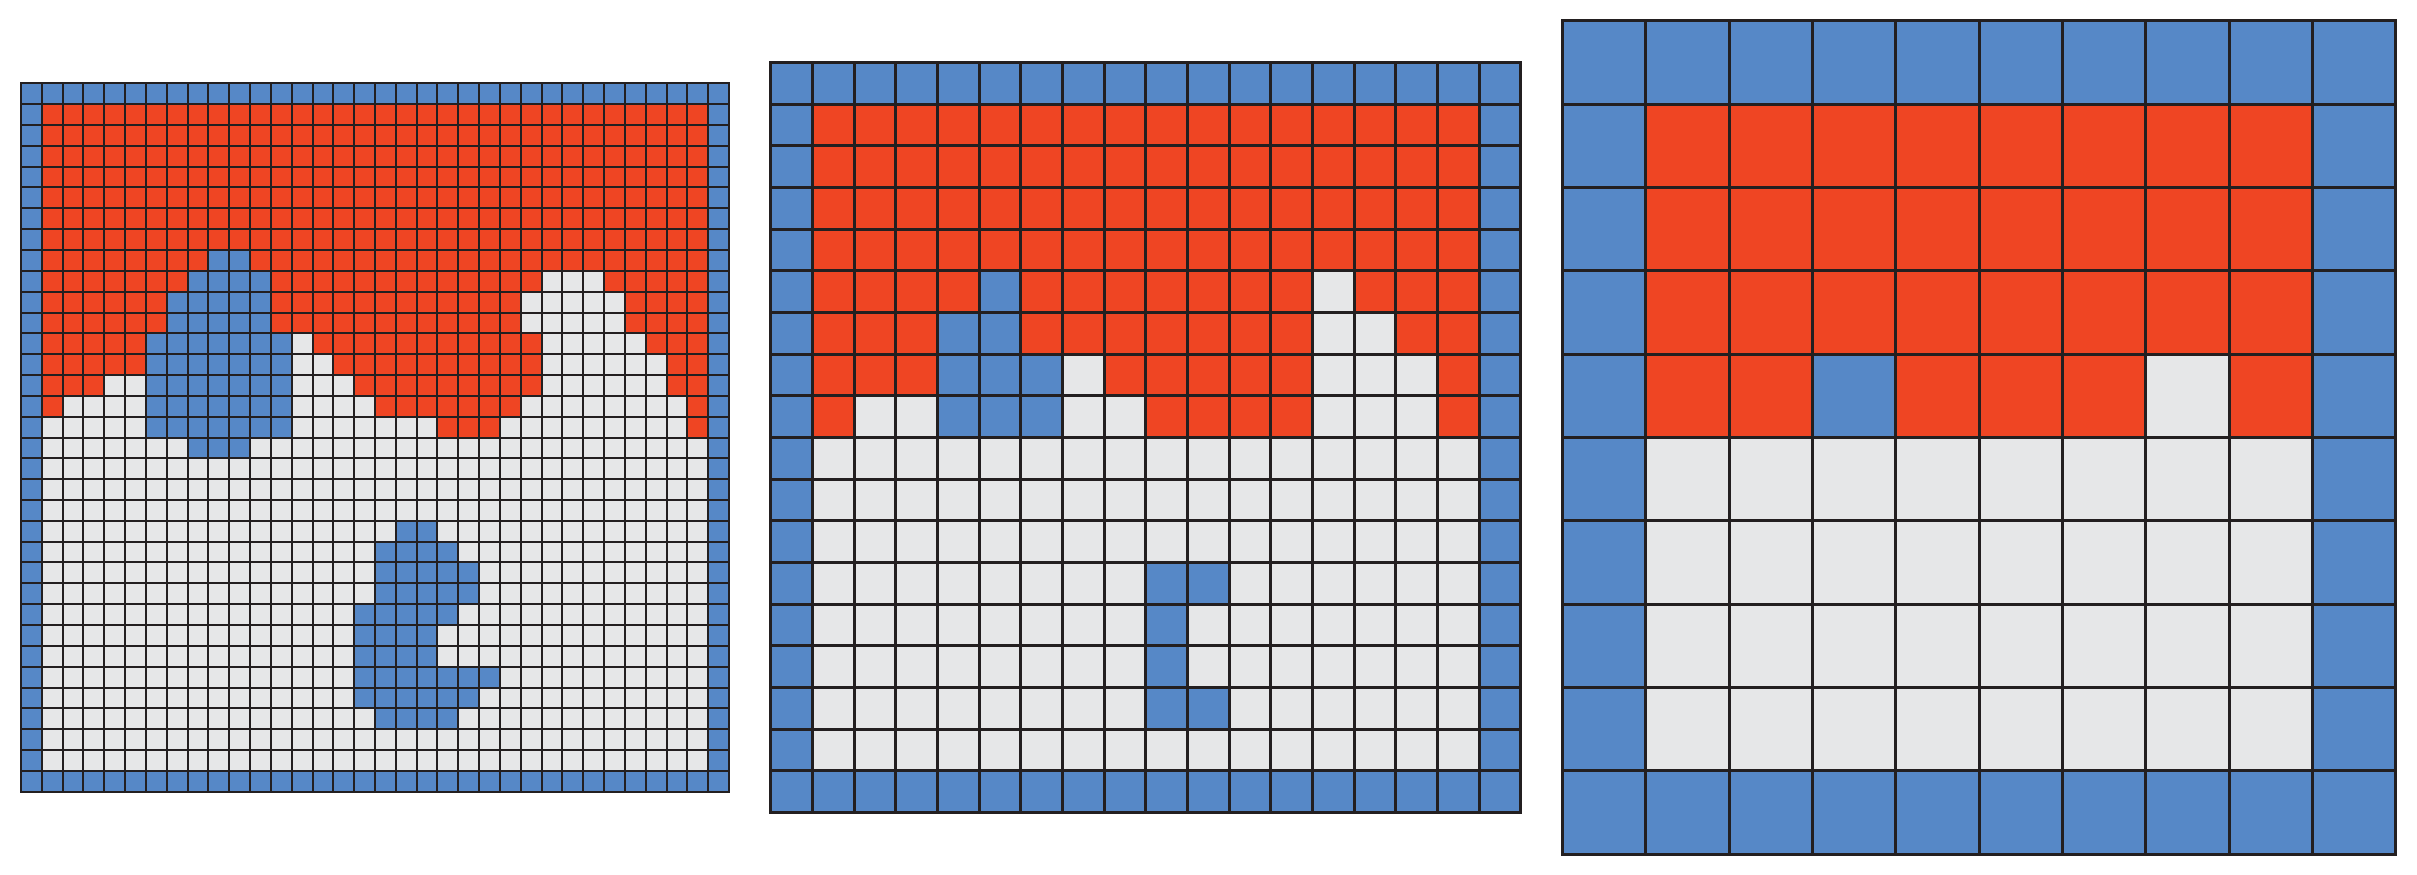
\includegraphics[width=1.05\columnwidth]{poisson/figures/refinement_illustration.pdf}}
\caption{Illustration of our coarsening strategy. Note the geometric and topological discrepancy between different resolution levels.}
\label{fig_refinement_illustration}
\end{figure}

\subsection{Multigrid cycle}
\label{sec_cycle}
We describe a geometric multigrid method for the Poisson problem defined in (\ref{eqn_problem}). Our approach uses a V-Cycle of the Multigrid Correction Scheme
\cite{trottenberg:2001:multigrid} and the pseudocode for each V-Cycle iteration is given in Algorithm \ref{alg_vcycle}. The V-Cycle procedure requires a discretization of the Poisson
problem at $L$$+$$1$ levels of resolution, denoted $\mathcal{L}^{(0)},\mathcal{L}^{(1)},\ldots,\mathcal{L}^{(L)}$, where level $0$ is at the finest resolution and level $L$ is the
coarsest. We also define a smoother at every level of the hierarchy and restriction/prolongation operators for transferring data across resolutions.

\begin{algorithm}[h]
\caption{V-Cycle of the Multigrid Correction Scheme.
\textit{Setting the initial guess to zero (line 2) is only necessary when the V-Cycle is used as a preconditioner. When the
  V-Cycle is used as an iterative solver line 2 should be omitted.}}
\label{alg_vcycle}
\begin{algorithmic}[1]
\Procedure{V-Cycle}{$\vec{u}^{(0)},\vec{b}^{(0)}$}\Comment{total of $L$$+$$1$ levels}
\State {\color{red}$\vec{u}^{(0)}\gets \vec{0}$}
\For{$l= 0 \textbf{\ to\ }L$$-$$1$}
\State Smooth($\mathcal{L}^{(l)}$,$\vec{u}^{(l)}$,$\vec{b}^{(l)}$)
\State $\vec{r}^{(l)}\gets\vec{b}^{(l)}-\mathcal{L}^{(l)}\vec{u}^{(l)}$
\State $\vec{b}^{(l+1)}\gets$Restrict($\vec{r}^{(l)}$),\ $\vec{u}^{(l+1)}\gets 0$
\EndFor
\State Solve $\vec{u}^{(L)}\gets (\mathcal{L}^{(L)})^{-1}\vec{b}^{(L)}$
\For{$l=L$$-$$1 \textbf{\ down to\ } 0$}
\State $\vec{u}^{(l)}\gets \vec{u}^{(l)}+$Prolongate($\vec{u}^{(l+1)}$)
\State Smooth($\mathcal{L}^{(l)}$,$\vec{u}^{(l)}$,$\vec{b}^{(l)}$)
\EndFor
\EndProcedure
\end{algorithmic}
\end{algorithm}

Our approach is purely geometric: at every level of the multigrid hierarchy we construct a voxelized description of our domain, classifying each cell as interior, Dirichlet or
Neumann. The procedure of Section \ref{sec_discretization} is then followed to construct a discrete Poisson operator $\mathcal{L}$ from this voxelized representation. The background
lattice for each coarser level of the hierarchy is constructed following a standard 8-to-1 cell coarsening procedure, generating a grid with twice the step size. Our hierarchy is deep: the coarsest level is typically $8\times8\times8$. The coarse grid is
positioned in such a way that the bounding box of the domain, excluding the ghost layer of Neumann cells, aligns with cell boundaries at both resolutions (see Figure
\ref{fig_refinement_illustration}). A coarse cell will be labeled Dirichlet, if any of its eight fine children is a Dirichlet cell. If none of the eight children is a Dirichlet cell, but at least one is
interior, then the coarse cell will be labeled as interior. Otherwise, the coarse cell is labeled Neumann. As seen in Figure \ref{fig_refinement_illustration} this coarsening strategy
can create significant geometric discrepancies when fine grid features are not resolved on the coarse, and even change the topology of the domain, e.g., Neumann bubbles are eventually
absorbed into the interior region, and thin interior features are absorbed into the Dirichlet region. The impact of this discrepancy is addressed later in this section.

We construct the restriction operator as the tensor product stencil $\mathcal{R}\!=\!\mathcal{B}\otimes\mathcal{B}\otimes\mathcal{B}$, where $\mathcal{B}$ is a 1D stencil with 4 points
given by:
\begin{align*}
&(\mathcal{B}\vec{u}^h)(x)=\mbox{$\frac{1}{8}$}u^h(x\mbox{$-$}\mbox{$\frac{3h}{2}$})+\mbox{$\frac{3}{8}$}u^h(x\mbox{$-$}\mbox{$\frac{h}{2}$})+\hspace*{.6in}&\\
&\hspace*{.6in}+\mbox{$\frac{3}{8}$}u^h(x\mbox{$+$}\mbox{$\frac{h}{2}$})+\mbox{$\frac{1}{8}$}u^h(x\mbox{$+$}\mbox{$\frac{3h}{2}$})=u^{2h}(x)&
\end{align*}
Figure \ref{fig_transfer_stencils} (left) illustrates the 2D analogue of this tensor product stencil, spanning 16 points (compared to 64, in 3D). Note that since our variables are cell
centered, the coarse grid variables will not coincide with a subset of the fine variables. The prolongation operator is defined by
$\mathcal{P}^T\!=\!8\mathcal{B}\otimes\mathcal{B}\otimes\mathcal{B}$, i.e., a scaled transposition of the restriction operator. We can verify that the prolongation is exactly a trilinear
interpolation operator from the coarse to the fine grid variables. We limit the output of the prolongation and restriction operators to interior cell variables only; therefore, we only
restrict into interior coarse cells, and only prolongate into interior fine variables. Conversely, if a restriction/prolongation stencil uses a non-interior cell variable as input, we
substitute a zero value instead.
%% In practice, we enforce that variables being restricted or prolongated will have zero values at non-interior cells; as a consequence the same restriction/prolongation stencils can be
%% used throughout the domain, without a need to modify these stencils near the boundary.

Our smoother of choice is the damped Jacobi method with parameter $\omega\!=\!^2\!\!/\!_3$ (see Algorithm \ref{alg_smoothers}), which is known to be stable for the Poisson equation and
facilitates parallelism better than Gauss-Seidel methods. For problems with mixed boundary conditions and irregular domain geometries it is common practice to perform additional
smoothing near the boundary of the computational domain. Consequently, we define a \emph{boundary region} consisting of interior cells within a certain distance of Dirichlet or Neumann
cells. Figure \ref{fig_transfer_stencils} (right) illustrates the boundary region (shaded black) within a radius of 2 of non-interior cells (measured by $L_1$-distance). In our approach,
we perform a number of Gauss-Seidel iterations (see Algorithm \ref{alg_smoothers}, bottom) on the boundary region in addition to the damped Jacobi smoother applied on the entire
domain. Our complete smoothing procedure will start with $M$ Gauss-Seidel sweeps on the boundary region, continue with a damped Jacobi sweep over the entire domain, and finish
with another $N$ Gauss-Seidel boundary sweeps. Finally, we can approximate the exact solution for the coarsest level in the hierarchy by simply iterating the smoothing procedure a large
number of times.

%% \vspace*{-.1in}
\begin{figure}[t]
\center{\hspace*{-.025\columnwidth}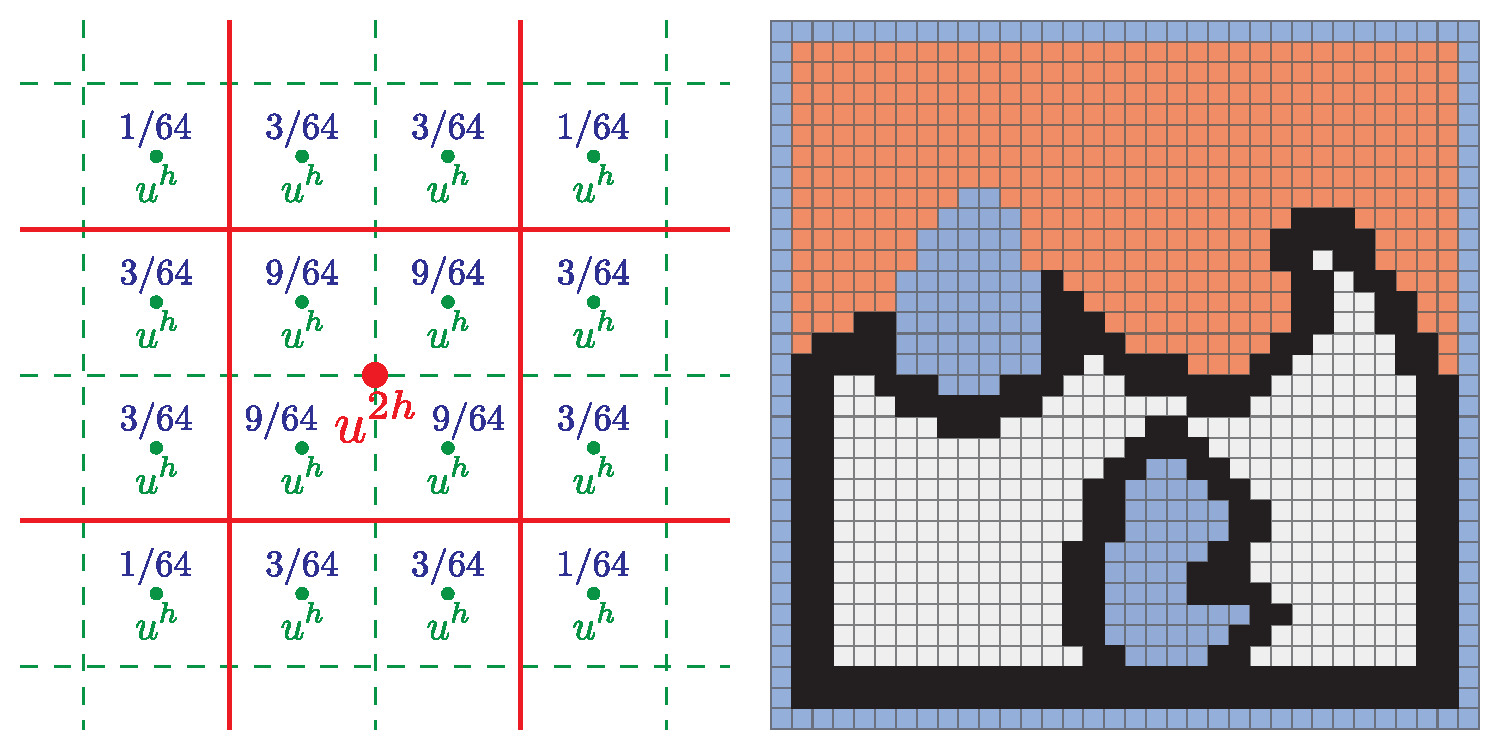
\includegraphics[width=1.05\columnwidth]{poisson/figures/transfer_stencils2.pdf}}
\caption{Left: 2D illustration of the restriction operator. Right: Illustration of the boundary region. A band width of 2 is pictured.}
\label{fig_transfer_stencils}
%% \vspace*{-.2in}
\end{figure}

\begin{algorithm}[h]
\caption{Damped Jacobi $(\omega\!=\!2/3)$ and Gauss-Seidel Smoothers}
\label{alg_smoothers}
\begin{algorithmic}[1]
\Procedure{DampedJacobiSmooth}{$\mathcal{L},\vec{u},\vec{b},\mathcal{I}$}
\State \textbf{foreach} $I=(i,j,k)\in\mathcal{I}$ \textbf{do}\Comment{$\mathcal{I}$ is set of cell indices}
\State \hspace*{1.em}$\delta_I\gets(b_I-\mathcal{L}_I\vec{u})/\mathcal{L}_{II}$\Comment{$\mathcal{L}_I$ is the equation in cell $I$}
\State \textbf{foreach} $I=(i,j,k)\in\mathcal{I}$ \textbf{do}
\State \hspace*{1.em}$u_I\plusequals\frac{2}{3}\delta_I$\Comment{$\boldsymbol{\delta}$ is an auxiliary variable}
\EndProcedure
\Procedure{GaussSeidelSmooth}{$\mathcal{L},\vec{u},\vec{b},\mathcal{I}$}
\State \textbf{foreach} $I=(i,j,k)\in\mathcal{I}$ \textbf{do}
\State \hspace*{1.em}$u_I\plusequals(b_I-\mathcal{L}_I\vec{u})/\mathcal{L}_{II}$
\EndProcedure
\end{algorithmic}
\end{algorithm}




The multigrid scheme we just described is particularly simplistic, using an elementary coarsening strategy, a very basic smoother and without specialized transfer operators near the
boundary. Not surprisingly, attempting to use this V-Cycle as an iterative solver for the Poisson problem reveals the following shortcomings:

\noindent\textbf{Instability:} When using multigrid as the solver instead of a preconditioner, the iterates produced by the sequence of V-Cycles can become highly oscillatory or divergent unless a substantial smoothing effort is spent near the
boundary. Specifically, we found it necessary to perform at least 30-40 iterations of boundary smoothing (15-20 iterations before the interior sweep, and 15-20 after) on a boundary band
at least 3 cells wide, in order to make the V-Cycle iteration stable for highly irregular domains. In contrast, a regular rectangular box domain with all Dirichlet boundary conditions
required only 2-3 boundary iterations on a boundary band just a single cell wide to remain perfectly stable with a $0.46$ convergence rate. This sensitivity to the regularity of the
domain is justified given the geometric discrepancies between different levels for irregular domains, and the imprecision of the transfer operators near the boundary, as discussed in \cite{trottenberg:2001:multigrid}. We will show that this sensitivity to the boundary treatment is removed when the V-Cycle is used as a preconditioner.

\noindent\textbf{Stagnation:} Even when the V-Cycle iteration is stable, on certain irregular domains the residual reduction rate quickly degrades towards 1, as opposed to converging to a value
less than 0.5 as typically expected of functional multigrid schemes. This complication appears on irregular domains where successive levels of the multigrid hierarchy may exhibit
significant topological differences, as coarse modes may not be accurately represented.  In these cases,  costly eigenanalysis or recombined iterants may prove useful \cite{trottenberg:2001:multigrid}; however, the highly irregular and changing domains common to fluid simulations make these methods impractical.

\subsection{Multigrid-preconditioned conjugate gradient}
\label{subsec_mgpcg}
The instability and slow convergence issues described in the previous section can be efficiently ameliorated by using the multigrid V-Cycle as a preconditioner for an appropriate Krylov method. 
Our experiments indicated that the elementary multigrid scheme in section \ref{sec_cycle} can be an extremely efficient preconditioner, achieving
convergence rates comparable or superior to the ideal performance of the V-Cycle on regular domains, even if the smoothing effort vested in the multigrid V-Cycle is significantly less than what is necessary
to make it a convergent solver on its own.

We will use the V-Cycle described in Section \ref{sec_cycle} as a preconditioner for the conjugate gradient method. Algorithm \ref{alg_mgpcg} provides the pseudocode for our PCG solver. Our
algorithm is numerically equivalent to the traditional definition of PCG, as stated for example in \cite{GolubVanLoan:1989:MC}, but certain variables are being reused for economy of
storage, and operations have been rearranged to facilitate optimized execution, as discussed in Section \ref{sec_implementation}. Preconditioning operates by constructing a symmetric,
positive definite matrix $\mathcal{M}$ which is easier to invert than $\mathcal{L}$, and such that $\mathcal{M}^{-1}\mathcal{L}$ is significantly better conditioned than
$\mathcal{L}$. 

%% The action of PCG on the system $\mathcal{L}\vec{u}=\vec{b}$ is equivalent to using the standard conjugate gradient method on the system $\mathcal{C}^{-1}\!\mathcal{L}\ \mathcal{C}^{-1}\vec{\hat{u}}=\mathcal{C}^{-1}\vec{b}$, where $\vec{u}=\mathcal{C}^{-1}\vec{\hat{u}}$ and the symmetric positive definite matrix $\mathcal{C}$ satisfies $\mathcal{M}=\mathcal{C}^2$ (existence of $\mathcal{C}$ is guaranteed by the symmetry and definiteness of $\mathcal{M}$).

In our case, we will use the multigrid V-Cycle as the preconditioner $\mathcal{M}^{-1}$ as described in \cite{T93}. In particular, if we define $\vec{u}:=\mathcal{M}^{-1}\vec{b}$, then
$\vec{u}$ is the result of one iteration of the multigrid V-Cycle for the problem $\mathcal{L}\vec{u}=\vec{b}$ \emph{with zero initial guess, and zero boundary conditions}. We can easily
verify that under these conditions, the action of the V-Cycle indeed corresponds to a linear operator; the requirement that $\mathcal{M}$ be symmetric and positive definite, however, is
less trivial. We refer to \cite{T93} for a detailed analysis of the conditions for symmetry and definiteness, and only present here a set of sufficient conditions instead. The V-Cycle of
Algorithm~\ref{alg_vcycle} will produce a symmetric and definite preconditioner if:

%% \vspace*{-.03in}
\noindent$\bullet$ The restriction/prolongation operators are the transpose of one another (up to scaling). This is common practice, and also the case for the V-Cycle we described.

%% \vspace*{-.03in}
\noindent$\bullet$ The smoother used in the \emph{upstroke} of the V-Cycle (Algorithm~\ref{alg_vcycle}, line 11) performs the operations of the smoother used for the \emph{downstroke} (line 4) in reverse
  order. E.g., if Gauss-Seidel iteration is used, opposite traversal orders should be used when descending or ascending the V-Cycle, respectively. For Jacobi smoothers, no
  reversal is necessary as the result is independent of the traversal order.

%% \vspace*{-.03in}
\noindent$\bullet$ The solve at the coarsest level (Algorithm~\ref{alg_vcycle}, line 8) needs to either be exact, or the inverse of $\mathcal{L}^{(L)}$ should be approximated with a symmetric and
  definite matrix. If the smoother is iterated to approximate the solution, a number of iterations should be performed with a given traversal order, followed by an equal number of
  iterations with the order reversed.

%% \begin{itemize}
%% \item The restriction/prolongation operators are the transpose of one another (up to scaling). This is common practice, and also the case for the V-Cycle we described, although it is not
%%   a prerequisite for multigrid methods, in general (e.g. \cite{brandt:1977:multilevel} uses non-adjoint transfer operators for the Poisson equation).
%% \item The smoother used in the \emph{upstroke} if the V-Cycle (Algorithm~\ref{alg_vcycle}, line 11) performs the operations of the smoother used for the \emph{downstroke} (line 4) in reverse
%%   order. For example, if Gauss-Seidel iteration is used, opposite traversal orders need to be used when descending or ascending the V-Cycle, respectively. For Jacobi smoothers, no
%%   reversal is necessary since the result is independent of the traversal order.
%% \item The solve at the coarsest level (Algorithm~\ref{alg_vcycle}, line 8) needs to either be exact, or the inverse of $\mathcal{L}^{(L)}$ should be approximated with a symmetric and
%%   definite matrix. If the smoother is iterated to approximate the solution, a number of iterations should be performed with a given traversal order, followed by an equal number of
%%   iterations with the order reversed.
%% \end{itemize}

%% \vspace*{-.1in}

\begin{algorithm}[h]
\caption{Multigrid-preconditioned conjugate gradient.
%%  \newline \it
 \textit{Red-colored steps in the algorithm are applicable when the Poisson problem has a nullspace (i.e., all
  Neumann boundary conditions), and should be omitted when Dirichlet boundaries are present.}
  \newline $(\dag)$ $\vec{u}\gets\mathcal{M}^{-1}\vec{b}$ is implemented by calling {
%%\sc
 V-Cycle}$(\vec{u},\vec{b})$}
\label{alg_mgpcg}
\begin{algorithmic}[1]
\Procedure{MGPCG}{$\vec{r},\vec{x}$}
\State $\vec{r}\gets\vec{r}-\mathcal{L}\vec{x},\ {\color{red}\mu\gets\bar{\vec{r}},}\ \nu\gets\|{\vec{r}\color{red}-\mu}\|_{\infty}$
\State \textbf{if} {$(\nu<\nu_{\max})$} \textbf{then return}
\State ${\color{red}\vec{r}\gets\vec{r}-\mu,}\ \vec{p}\gets\mathcal{M}^{-1}\vec{r}^{(\dag)},\ \rho\gets\vec{p}^T\vec{r}$
\For{$k= 0 \textbf{\ to\ }k_{max}$}
\State $\vec{z}\gets\mathcal{L}\vec{p},\ \sigma\gets\vec{p}^T\vec{z}$
\State $\alpha\gets\rho/\sigma$
\State $\vec{r}\gets\vec{r}-\alpha\vec{z},\ {\color{red}\mu\gets\bar{\vec{r}},}\ \nu\gets\|{\vec{r}\color{red}-\mu}\|_{\infty}$
\If{$(\nu<\nu_{\max}$ \textbf{or} $k=k_{\max})$}
\State $\vec{x}\gets\vec{x}+\alpha\vec{p}$
\State \textbf{return}
\EndIf
\State ${\color{red}\vec{r}\gets\vec{r}-\mu,}\ \vec{z}\gets\mathcal{M}^{-1}\vec{r}^{(\dag)},\ \rho^{\mbox{new}}\gets\vec{z}^T\vec{r}$
\State $\beta\gets\rho^{\mbox{\small new}}/\rho$
\State $\rho\gets\rho^{\mbox{\small new}}$
\State $\vec{x}\gets\vec{x}+\alpha\vec{p},\ \vec{p}\gets\vec{z}+\beta\vec{p}$
\EndFor
\EndProcedure
\end{algorithmic}
\end{algorithm}

Finally, Poisson problems with all-Neumann boundary conditions (e.g., simulations of smoke flow past objects) are known to possess a nullspace, as the solution is only known up to a
constant. The algorithm of Algorithm~\ref{alg_mgpcg} is modified in this case to project out this nullspace, and the modifications are highlighted in red in the pseudocode. No modification
to the V-Cycle preconditioner is needed.

% \vspace*{-.05in}
\section{Implementation and Optimizations}
 %\vspace*{-.05in}
\label{sec_implementation}

%% The simplicity of the V-Cycle enabled extensive optimizations and software tuning for parallel execution on shared memory
%% computers. These implementation strategies are detailed below.

\textbf{Minimizing boundary cost:} The cost of performing 30-40 smoothing sweeps on the boundary to stabilize the V-Cycle as a solver cannot be neglected, even though the interior
smoothing effort would asymptotically dominate. In practice, this amount of boundary smoothing would be the most costly operation of the V-Cycle for a $256^3$ grid or smaller, assuming serial
execution. For parallel execution, boundary smoothing would be the clear bottleneck for even higher resolutions ($512^3$ or more in practice) since the boundary smoother has inferior
scalability to the interior smoother due to the irregularity of the boundary band. Since in our approach the V-Cycle will only be used as a CG preconditioner, we do not need to spend
that much effort smoothing the boundary. Our experiments indicated that even with no extra smoothing near the boundary the PCG algorithm would be stable and convergent, but only with a
moderate acceleration over the unpreconditioned CG method. However, the following carefully designed boundary smoothing led to very rapid convergence.

%We used the following rule for determining the extent of the boundary region: An interior cell will be included in the boundary region if the restriction operation transfers the value of
%this cell to a non-interior coarse variable. Equivalently, an interior cell is included in the boundary band if its prolongation from the coarse grid includes non-interior coarse
%variables. 
The extent of our boundary region depends on our prolongation operator as well as our standard 8-to-1 coarsening scheme. Define $D(\mathcal{P},I^{(l)})$ as the set of coarse cells in the prolongation stencil of an interior cell $I^{(l)}$.  For each $I^{(l+1)}\in D(\mathcal{P},I^{(l)})$, if any of its 8 fine children are not interior cells, $I^{(l)}$ is included in the boundary band.
This heuristic produces a boundary region with a width up to 3 cells (near irregular interfaces) or as low as 1 cell (near walls and boundaries resolved by all grids).
%% We found that including fewer cells than determined by this rule in the boundary band would decelerate PCG convergence, while including more tends to have diminishing returns (and
%% necessitate more boundary iterations). 
Additionally, we only perform boundary smoothing \emph{after} the interior sweep on the downstroke of the V-Cycle and \emph{before} the interior
sweep on the upstroke. 
%%As a result, the extra boundary smoothing always occurs between the inter-grid transfer and the interior smoothing sweep.
We found that using 2 Gauss-Seidel
iterations on the boundary band at the finest level struck the best balance of computational cost and PCG efficiency. 
%% Naturally, the traversal order of the Gauss-Seidel sweep was
%% reversed between the downstroke and upstroke of the V-Cycle, to ensure symmetry.
Since the size of the boundary band at every coarser level is reduced by a factor of four, we
increase the number of boundary sweeps by a factor of 2 every level (i.e., performing $2^{l+1}$ sweeps at level $l$), which incurs only a minimal overhead but further accelerates convergence.

%% \vspace*{-.05in}
\noindent\textbf{Compact representation of $\mathcal{L}$:} The discrete operator $\mathcal{L}$ contains the standard 7-point stencil in the interior of the domain, with a
coefficient of $-6/h^2$ on the center cell and $1/h^2$ on the 6 face neighbors. We can eliminate the $1/h^2$ factor by observing that the preconditioning ability of $\mathcal{M}^{-1}$
remains unchanged if the entire matrix is scaled. Thus, if we consider the V-Cycle to be a solver for $h^2\Delta$ instead of the unscaled Poisson operator, the operator
coefficients at the interior of the finest level simply become $-6$ and $1$. 
%%Of course, this $h^2$-scaling will not eliminate the denominators for the coarser grids; however, 
If we
modify the prolongation operator as $\mathcal{P}^T\!=\!2\mathcal{B}\otimes\mathcal{B}\otimes\mathcal{B}$, then the integer-valued
scaled-Poisson stencils (with entries $-6$ and $1$) can be used at all levels of the hierarchy. This stencil will only assume a different form near Neumann boundaries: the scaled
7-point stencil will have a coefficient of 1 for any non-Neumann neighbors, a value of zero for Neumann neighbors, and the center coefficient will be the negative count of
non-Neumann neighbors. Instead of storing these zero Neumann coefficients, we enforce the condition that any variables where the discrete operator $\mathcal{L}$ will be applied to,
shall have zero values on any non-interior cells. As a consequence, we only need to store a negative integer (the center coefficient)  to represent the Poisson
operator near the boundary. 
%% In fact, we only store the central coefficient (and its inverse, needed in the smoothing routines) on flattened arrays with the size of the boundary
%% band, instead of storing them throughout the entire domain.

%% \vspace*{-.05in}
\noindent\textbf{Using zero initial guess and boundary conditions:} When the multigrid V-Cycle is used as a preconditioner, it is solving a Poisson problem with zero boundary conditions,
and uses a zero initial guess as discussed in Section \ref{subsec_mgpcg}. Also, every subsequent level of the multigrid correction scheme will also employ zero initial guess and
boundary conditions. This fact allows us to simplify and combine steps 2,4, and 5 of the algorithm in Algorithm~\ref{alg_vcycle}, which are the most costly components of the V-Cycle
algorithm. For simplicity, consider an all-Dirichlet problem, where $\mathcal{L}$ has the same 7-point stencil (with coefficients -6 and 1 as discussed before) everywhere in the
domain. Using the fact that $\vec{u}^{(0)}=\vec{0}$, line 3 of the damped Jacobi smoother in Algorithm~\ref{alg_smoothers} produces $\boldsymbol{\delta}=-\frac{1}{6}\vec{b}$ and the result of the
relaxation will be $\vec{u}=-\frac{1}{9}\vec{b}$. The residual after the relaxation will be
$\vec{r}=\vec{b}-\mathcal{L}(-\frac{1}{9}\vec{b})=\frac{1}{9}(\mathcal{L}+9\mathbf{I})\vec{b}$. Thus, both the smoothed solution $\vec{u}$ as well as the residual $\vec{r}$
resulting from this smoother can be computed simultaneously from $\vec{b}$, in a single streaming pass over these 3 variables ($\delta$ is just temporary and need not be computed).
Of course, this procedure will be invalid near Neumann boundaries, where $\mathcal{L}$ has a modified stencil. For this reason, we mask the output on $\vec{u}$ to exclude cells
with non-standard stencils, setting those values to zero instead. These cells will be smoothed in the boundary sweep immediately afterwards. Lastly, the Gauss-Seidel boundary
sweep will invalidate the residuals computed near the boundary band. We correct this by updating the residuals in the 1-ring of the boundary band at the end of the smoothing procedure.

%\begin{figure}[t]
%\center{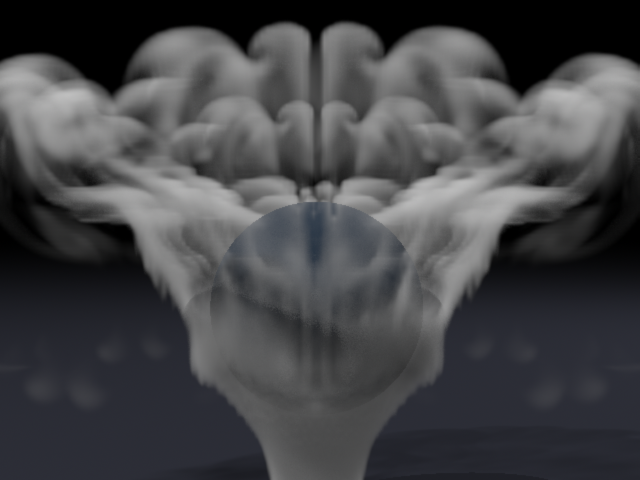
\includegraphics[width=.495\columnwidth]{poisson/figures/smoke_192_closeup_00090.png} 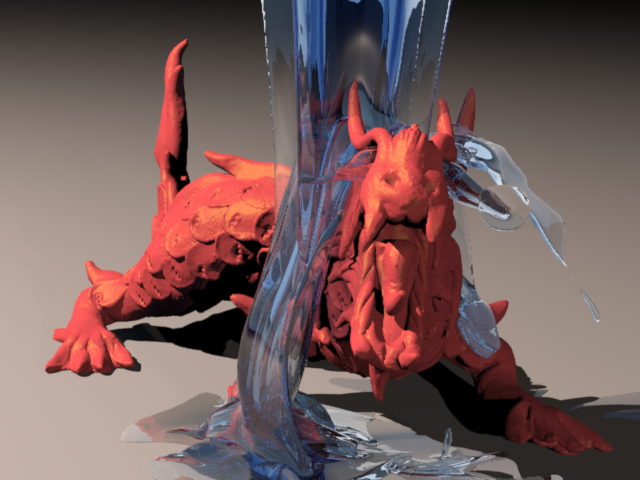
\includegraphics[width=.495\columnwidth]{poisson/figures/dragon_no_pool_closeup_00013.png}}\vspace*{.01in}
%\center{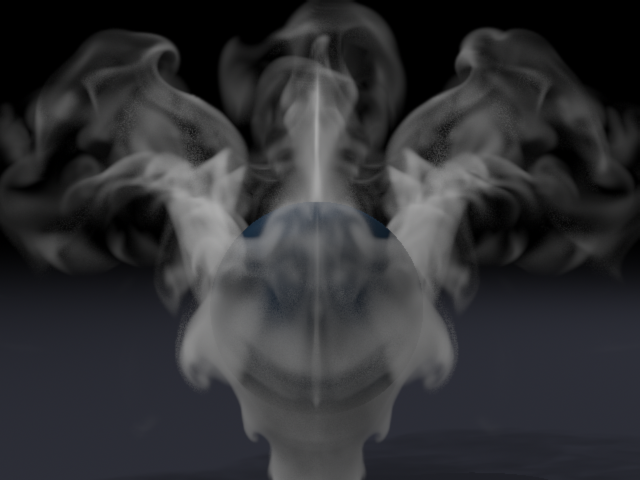
\includegraphics[width=.495\columnwidth]{poisson/figures/smoke_384_closeup_00090.png} 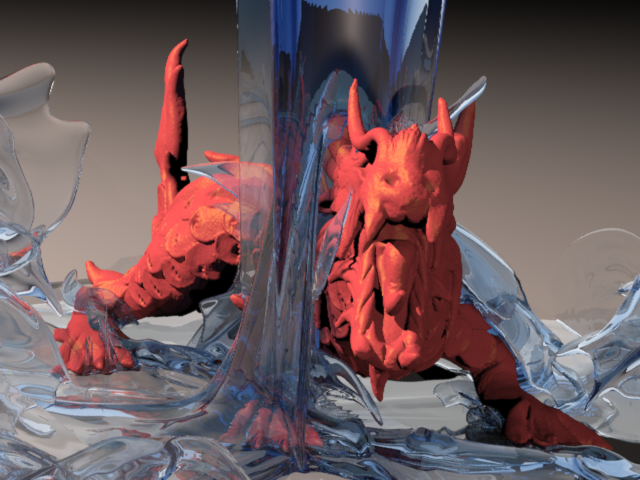
\includegraphics[width=.495\columnwidth]{poisson/figures/dragon_no_pool_closeup_00027.png}}\vspace*{.01in}
%\center{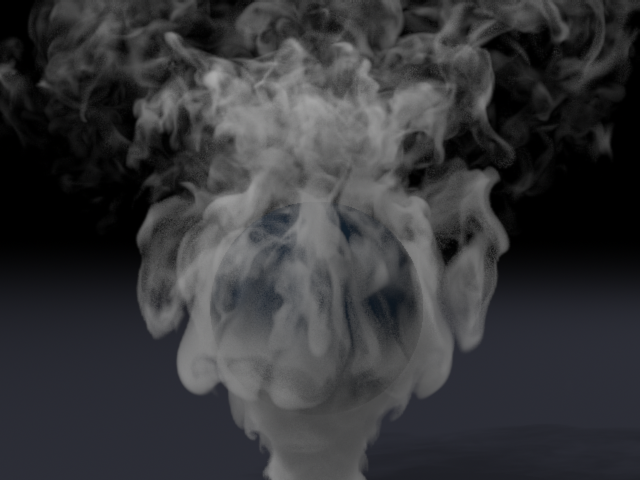
\includegraphics[width=.495\columnwidth]{poisson/figures/smoke_768_closeup_00090.png} 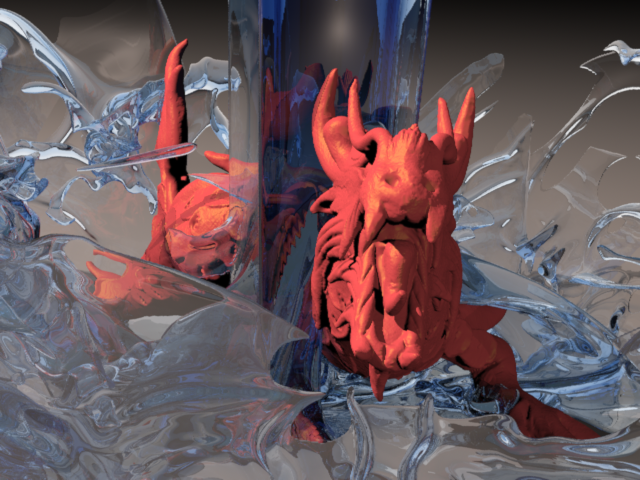
\includegraphics[width=.495\columnwidth]{poisson/figures/dragon_no_pool_closeup_00036.png}}
%%% \vspace*{-.25in}
%\caption{Left: Smoke plume simulation at resolutions of $192^2\times 288$ (top), $384^2\times 576$ (middle) and $768^2\times 1152$ (bottom). Right: Free surface water simulation on a $512^3$ grid.}
%%% \vspace*{-.25in}
%\label{fig_smoke_and_fire}
%\end{figure}

\noindent\textbf{Pipelining operations:} Streaming operations in the PCG algorithm  were often combined in a single pass through memory. The pseudocode in Algorithm~\ref{alg_mgpcg} has
been written to indicate such combinable operations on the same line, e.g., lines 2, 4, 6, 8, 13, and 16.
%% For example, in line 3 we compute a sum, maximum and minimum
%% $r_{\mbox{\small sum}}=\sum r_i, r_{\mbox{\small min}}=\min\{r_i\}, r_{\mbox{\small max}}=\max\{r_i\}$ as we compute the updated residuals $r_i$ in a streaming fashion. Constants
%% $\mu,\nu$ are computed at the end of the loop as $\mu=r_{\mbox{\small sum}}/N$ and $\nu=\max\{|r_{\mbox{\small min}}-\mu|,|r_{\mbox{\small max}}-\mu|\}$. We performed a similar
%% aggregation of all the vector operations listed on the lines mentioned.

%% \vspace*{-.06in}
\noindent\textbf{Multithreading:} Most of the operations in our solver are trivially parallelizable, as they are order independent (excluding the boundary smoother). In order to parallelize the boundary Gauss-Seidel smoother, we tiled the domain with blocks of size $4\times 4\times 4$ which were subsequently red-black
colored. Subsequently, we parallelize the Gauss-Seidel sweep over the red blocks, distributing a balanced number of blocks to each processor, without fine-grain locking. Black blocks are
processed in a separate parallel sweep. 
%% This process is followed in the V-Cycle downstroke; naturally, we first process black blocks, then red, in the upstroke (reversing the
%% Gauss-Seidel traversal order within blocks) to retain symmetry. 
Iterating the Gauss-Seidel smoother as many as 10 times within each block costs less than twice
the cost of a single iteration (due to cache effects) which further improved the efficiency of our preconditioner.

%% \vspace*{-.06in}
\noindent\textbf{Variable reuse and storage footprint:} Our methodology reuses vector variables to minimize the memory footprint. We only
require (and reuse) the following 5 vector variables, defined over the entire domain: $\vec{x}$ (for initial guess and solution), $\vec{r}$ (for initial right hand side, subsequent residuals and also
the right-hand side $\vec{b}^{(0)}$ at the top level of the V-Cycle), $\vec{p},\vec{z}$ (reused throughout CG, also used as the solution $\vec{u}^{(0)}$ at the finest V-Cycle level)
and $\boldsymbol{\delta}$ (reused to hold the residual $\vec{r}$ within the V-Cycle). Vector variables
for the coarser levels are smaller by a factor of 8. We also represent the extent of the interior/boundary regions using bitmaps
for a minor storage overhead (e.g., for the Jacobi smoother or transfer operators which are restricted to interior cells). Quantities such as the diagonal element of $\mathcal{L}$ (and
its inverse) are only stored for the boundary region. Ultimately, the entire PCG solver for a $768^2\times 1152$ grid has a memory footprint slightly under $16$GB (out of which, $12.8$GB
used for $\vec{x},\vec{r},\vec{p},\vec{z}$ and $\boldsymbol{\delta}$) and an entire smoke solver at this resolution fits easily in $32$GB of memory. We note that our method maintains minimal
metadata, and the memory for all data variables can be reused outside of the solver. For example, we have reused $\vec{p},\vec{z}$ and $\boldsymbol{\delta}$ in the
advection step to store the pre-projection velocities.

% \vspace*{-.05in}
\section{Examples}
% \vspace*{-.05in}
We demonstrate the efficacy of our solver with high resolution smoke and free surface simulations. We use simple semi-Lagrangian advection \cite{Stam:1999:SF} for the density and level
sets. Velocity extrapolation for air velocities was done as in \cite{zhu:2005:sand} and fast sweeping \cite{Z04} was used for level set reinitialization. Semi-Lagrangian advection 
is plagued by substantial numerical viscosity at lower resolutions; however, the efficiency and lightweight nature of our voxelized Poisson solver allows for sufficiently high resolution
to produce detailed incompressible flows with these comparably simple methods. Figure \ref{fig_smoke_and_fire} demonstrates the effect of the available resolution.  We found a tolerance of $\|r\|_{\infty}<10^{-3}$ for smoke simulations and and $10^{-5}$ for free surface produced visually pleasing results.
%% The smoke simulations
%% in the left column are done at top resolution of $768\times768\times1152$ and the free surface simulation at the right is done with $512^3$ resolution. 
%Although we used resolutions substantially higher than typical, the bulk of the computation was in advection and level set reinitialization rather than the voxelized Poisson solves (see
%Table~\ref{fig_runtimes}). 
Table~\ref{fig_runtimes} gives runtimes for the voxelized Poisson solves in our simulations.  Although we used resolutions substantially higher than typical, the Poisson solves represent between $25\%$ and $50\%$ of total simulation time. 
These examples demonstrate the solver's ability to handle rapidly changing domain geometries and to converge with just a few PCG iterations in practical
settings. 

Figure~\ref{fig_convergence} compares the convergence of our method with CG and incomplete Cholesky PCG in terms of rate per iteration. As incomplete Cholesky PCG involves sparse back-substitution and cannot be parallelized without significant effort (if at all), we compare serial runtimes for an incomplete Cholesky PCG implementation, a ``black-box'' conjugate gradient solver, our streamlined conjugate gradient solver, and our multigrid preconditioned solver to a given tolerance on the smoke past sphere domain in Table~\ref{fig_runtime_comparison}.  Even without the aid of parallelization, we see a $4.5\times$ speed-up at $128^3$ over ICPCG, a $10\times$ speed-up at $256^3$, and a $20\times$ speed-up at $512^3$ resolution.  Our ICPCG and ``black-box'' CG solvers are generic implementations with explicit compressed sparse row matrix representations.

% \vspace*{-.05in}
\section{Limitations and future work}
 %\vspace*{-.05in}
\label{sec_discussion}
Our performance at high resolutions is largely due to parallelization. While the convergence rate remains excellent, parallel scalability is inferior at lower resolutions. Our method was tuned
for shared-memory multiprocessors since we targeted problem sizes that would not fit on GPU memory. However, our method would benefit from the bandwidth of GPU platforms and we will
investigate GPU ports of our method as future work. Methods that approximate the domain with sub-cell accuracy could be expected to produce improved results for the same base resolution. The results of \cite{SW05} suggest methods such as
 \cite{BBB07} would likely be accelerated with a small adjustment to our method. The resolution enabled by our method could be combined with techniques such as wavelet turbulence
 \cite{KTJG08} or vorticity confinement \cite{FSJ01} to add even more detail. In the future, an adaptive multigrid formulation such as semicoarsening \cite{trottenberg:2001:multigrid}
 could also be used to precondition an adaptive method such as \cite{LGF04}, although obtaining the same level of scalability would be challenging in this context.

\begin{table}[tb]
 \center{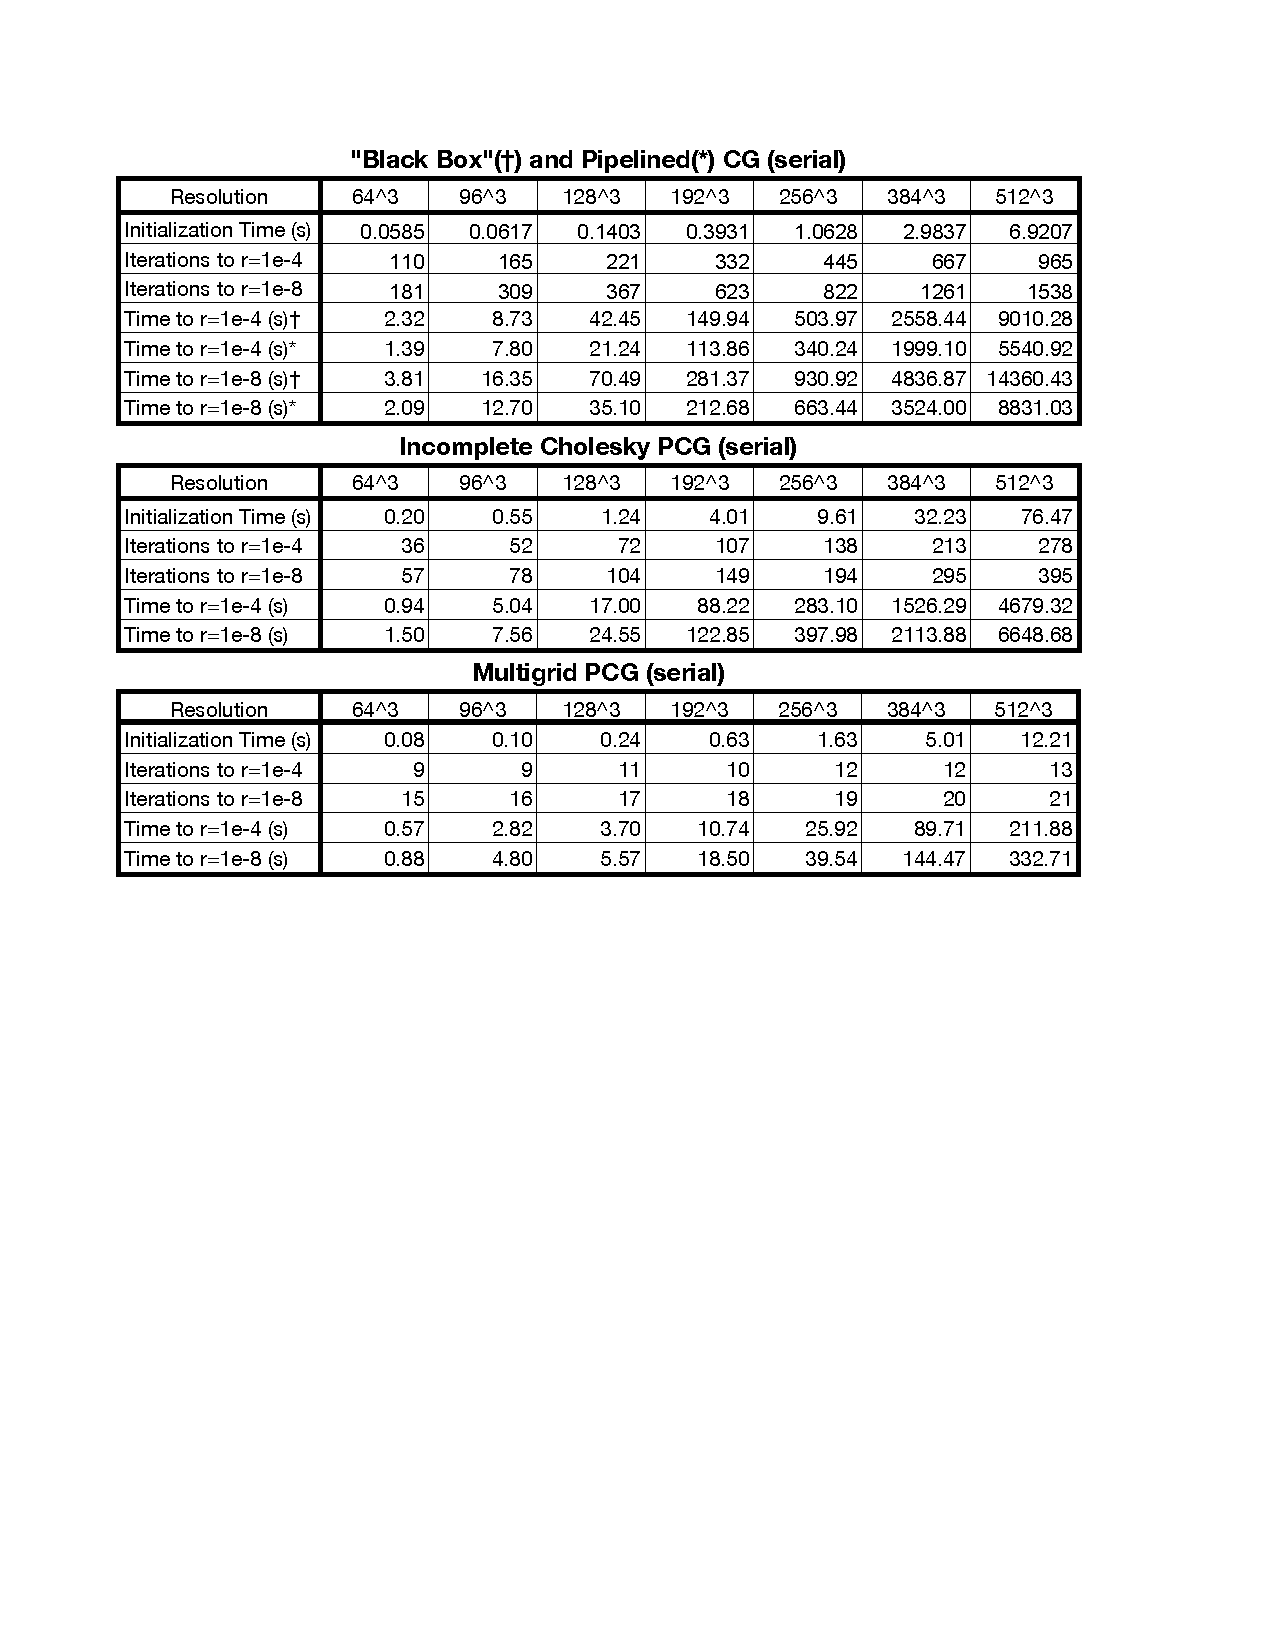
\includegraphics[width=\columnwidth]{poisson/figures/runtime_compare.pdf}}
 \caption{Number of iterations and \textbf{serial} runtimes for our modified conjugate gradient(*) and a ``black box''($\dagger$) solver (top), incomplete Cholesky PCG (middle), and our method (bottom).  Initialization time includes building any matrices and computing incomplete Cholesky factorization for ICPCG or building multigrid hierarchy for MGPCG.}\label{fig_runtime_comparison}
\end{table}


\begin{table}[tb]
\center{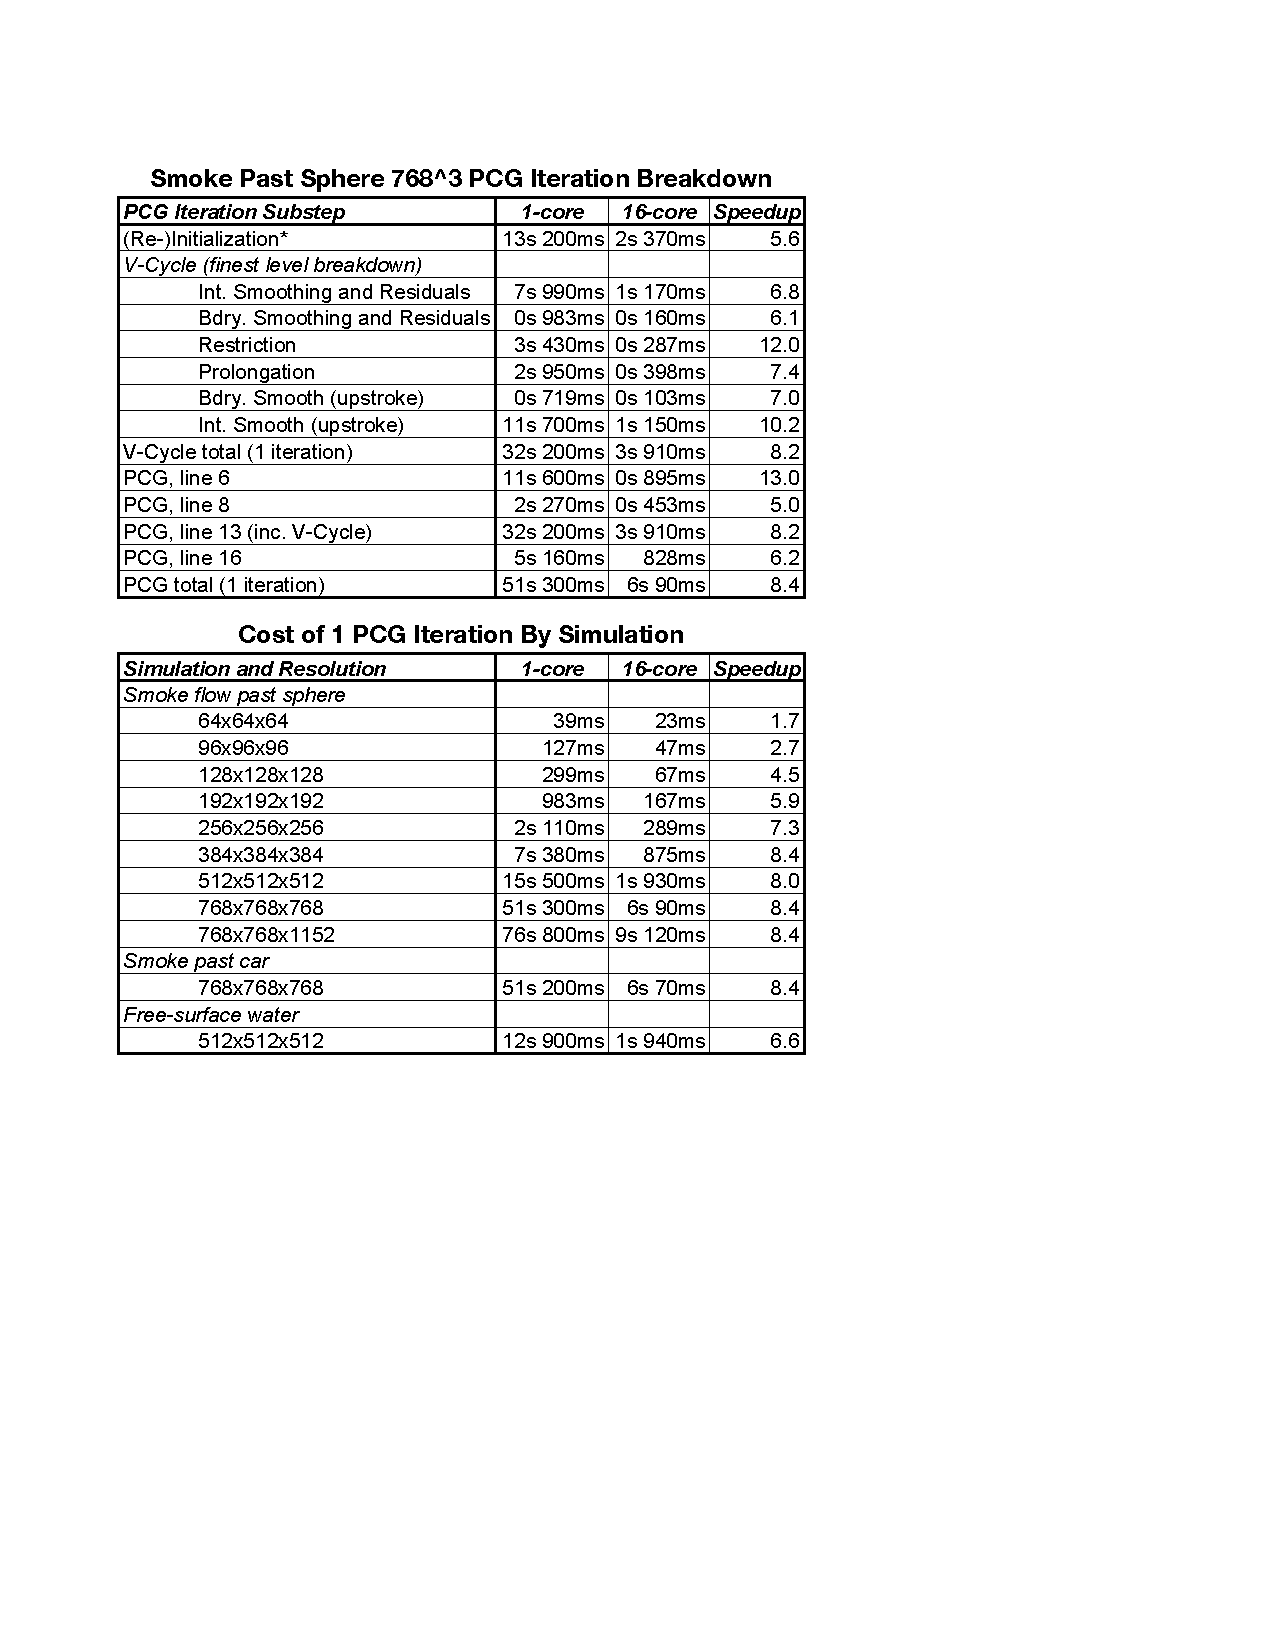
\includegraphics[width=\columnwidth]{poisson/figures/runtimes1.pdf}}
\caption{Execution cost and parallel speedup for our method. All parallel computations were carried out on a 16-core Intel Xeon X7350 server with 32GB of RAM. (*)Initialization refers to multigrid hierarchy initialization.}
\label{fig_runtimes}
\end{table}



\begin{figure}[tcb]
\center{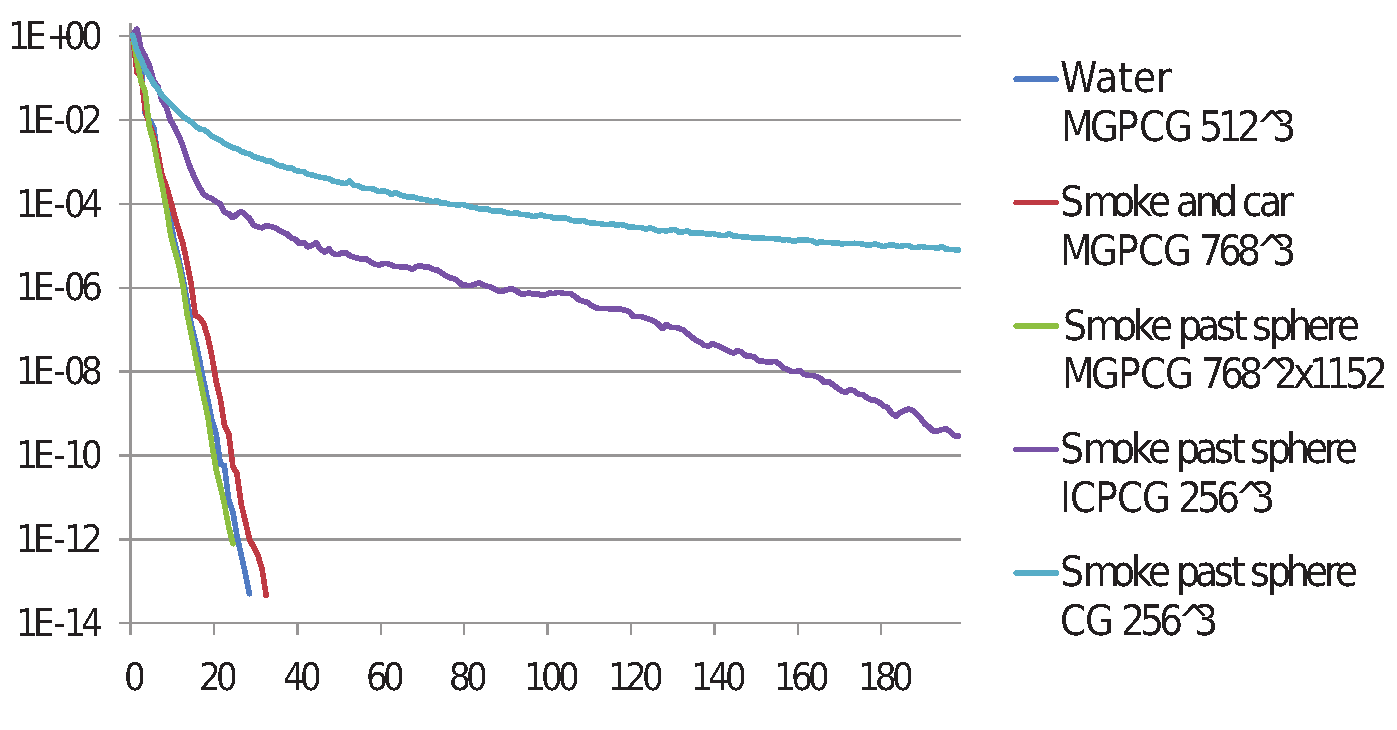
\includegraphics[width=\columnwidth]{poisson/figures/convergence.pdf}}
\caption{
Comparison of multigrid-preconditioned CG (MGPCG), incomplete Cholesky PCG (ICPCG) and unpreconditioned CG (CG).
The horizontal axis corresponds to iterations, the vertical indicates the residual reduction factor $|r_k|/|r_0|$ after $k$ iterations.
}
\label{fig_convergence}
\end{figure}
